\documentclass[11pt,aspectratio=43,compress]{beamer}
\usepackage{ruc-research}
\graphicspath{{assets/}}
\definecolor{ink}{HTML}{29252A}
\definecolor{slate}{HTML}{365E75}
\definecolor{quiet}{HTML}{555159}
\definecolor{papergray}{HTML}{F3F1F2}
\definecolor{paperrose}{HTML}{F6EAEC}
\definecolor{paperblue}{HTML}{EAF0F4}
\colorlet{wine}{tsinghua}
\setbeamercolor{normal text}{fg=ink,bg=white}
\setbeamercolor{title}{fg=wine,bg=white}
\setbeamerfont{frametitle}{size=\fontsize{15}{17}\selectfont}
\setbeamerfont{framesubtitle}{size=\small}
\setbeamertemplate{mini frames}[default]
\setbeamertemplate{page number in head/foot}[totalframenumber]
\setbeamercolor{result strip}{fg=wine!88!black,bg=paperrose}
\setbeamercolor{question strip}{fg=slate!80!black,bg=paperblue}
\newcommand{\strap}[1]{\par{\small\color{slate}\bfseries #1}\par\smallskip}
\newcommand{\finding}[1]{%
  \par\smallskip\begin{beamercolorbox}[wd=\linewidth,sep=5pt,rounded=false]{result strip}%
  \small #1\end{beamercolorbox}\par}
\newcommand{\nextq}[1]{%
  \par\smallskip\begin{beamercolorbox}[wd=\linewidth,sep=5pt,rounded=false]{question strip}%
  \small #1\end{beamercolorbox}\par}
\newcommand{\refnote}[1]{\par\smallskip{\fontsize{7.5}{9}\selectfont\color{quiet}#1\par}}
\newcommand{\greatnum}[1]{{\fontsize{27}{29}\selectfont\bfseries\color{wine}#1}}
\newcommand{\shortlabel}[1]{{\small\bfseries\color{slate}#1}}
\newcommand{\urllit}[1]{\texttt{#1}}
\setlength{\tabcolsep}{4pt}
\renewcommand{\arraystretch}{1.24}
\tikzset{
  storybox/.style={draw=quiet!25, fill=papergray, rounded corners=2pt, align=center,
    minimum height=1.12cm, inner sep=3pt, font=\small},
  storyfocus/.style={storybox, draw=wine!60, fill=paperrose},
  storyarrow/.style={-{Stealth[length=2mm]}, semithick, draw=quiet},
  grapharrow/.style={-{Stealth[length=2mm]}, semithick, draw=wine}
}
\title[个人投资者的信息集]{On the Information Set of\\Individual Investors}
\author[Laarits \& Wurgler]{Toomas Laarits \texorpdfstring{\quad}{and } Jeffrey Wurgler}
\institute[NYU Stern]{NYU Stern School of Business}
\date{2026年4月27日工作稿}
\begin{document}
\begin{frame}[plain]
  \vfill
  {\small\color{wine}\bfseries 科研组会\par}
  \vspace{5mm}
  {\fontsize{22}{26}\selectfont\bfseries
   On the Information Set of\\Individual Investors\par}
  \vspace{3mm}
  {\large\color{wine}个人投资者的信息集\par}
  \vspace{3mm}
  {\color{wine}\rule{.95\linewidth}{.75pt}}\par
  \medskip
  Toomas Laarits \quad Jeffrey Wurgler\par
  {\small NYU Stern School of Business \hfill 2026年4月27日工作稿}
  \vfill
\end{frame}

\section{研究问题}
\subsection{1.1 信息输入}
\begin{frame}{同一笔买入，背后看过什么？}
  \strap{1.1\quad 理论需要什么信息输入}
  \begin{center}
    \begin{tikzpicture}
      \node[storybox,text width=2.12cm] (menu) {可得资料\\[-1pt]\scriptsize 行情、财报};
      \node[storyfocus,text width=2.12cm,right=5mm of menu] (see) {\textbf{在线获取}\\[-1pt]\scriptsize 股票、内容、时点};
      \node[storybox,text width=2.12cm,right=5mm of see] (belief) {形成判断\\[-1pt]\scriptsize 预期与风险认识};
      \node[storybox,text width=1.65cm,right=5mm of belief] (trade) {买卖\\[-1pt]\scriptsize 订单事件};
      \draw[storyarrow] (menu)--(see);
      \draw[storyarrow] (see)--(belief);
      \draw[storyarrow] (belief)--(trade);
    \end{tikzpicture}
  \end{center}
  \vspace{2mm}
  \begin{columns}[T,onlytextwidth]
    \column{.48\textwidth}\shortlabel{家庭甲}\par 查盈利预测后买入。
    \column{.48\textwidth}\shortlabel{家庭乙}\par 查看近期价格后买入。
  \end{columns}
  \finding{本文测量在线信息获取，再用订单时点把研究放回交易情境。}
  \refnote{决策链为概念示意，甲乙为教学例。论文 pp.~2–3、10–11。}
\end{frame}

\begin{frame}{模型对所需信号给出不同答案}
  \strap{1.1\quad 理论需要什么信息输入}
  \begin{tabularx}{\linewidth}{@{}L{.27\linewidth}YY@{}}
    \toprule
    \textbf{理论视角} & \textbf{模型中的输入} & \textbf{对应的经验问题}\\
    \midrule
    组合选择 & 收益分布与协方差 & 是否查过可用于判断风险的资料？\\
    信息扩散 & 新闻与价格走势 & 哪些人接触了哪类内容？\\
    收益外推 & 历史收益 & 实际看到多长的价格历史？\\
    \bottomrule
  \end{tabularx}
  \medskip
  \finding{个体获取了什么，决定理论中的信息输入能否与行为事实对接。}
  \refnote{理论线索据论文 pp.~2–3、6–7。市场价格反映信息属于另一个层面的经验问题。}
\end{frame}

\subsection{1.2 注意力证据}
\begin{frame}{搜索峰值之后，投资者打开了什么？}
  \strap{1.2\quad 已有注意力证据与本文增量}
  \begin{center}
  \begin{tikzpicture}
    \node[storybox,text width=2.5cm] (search) {某股搜索上升};
    \node[storyfocus,text width=3cm,right=18mm of search,yshift=8mm] (chart) {可能打开价格图};
    \node[storyfocus,text width=3cm,right=18mm of search,yshift=-8mm] (earn) {可能查盈利预测};
    \draw[storyarrow] (search.east)--(chart.west);
    \draw[storyarrow] (search.east)--(earn.west);
  \end{tikzpicture}
  \end{center}
  \begin{tabularx}{\linewidth}{@{}L{.24\linewidth}Y@{}}
    \textbf{搜索指数} & 看到哪些股票在什么时候引起关注。\\
    \textbf{单一券商活动} & 可连接账户行为，站外阅读未纳入同一轨迹。\\
    \textbf{本文的跨站浏览} & 能比较同一家庭访问的页面、内容与交易时点。\\
  \end{tabularx}
  \refnote{图为教学示意。相关文献与数据比较见论文 pp.~3、5–7、18–19。}
\end{frame}

\begin{frame}{把同一家庭的研究与交易连起来}
  \strap{1.2\quad 同一数据怎样产生四类比较}
  \begin{tabularx}{\linewidth}{@{}L{.30\linewidth}Y@{}}
    \toprule
    \textbf{记录提供什么} & \textbf{据此可以问什么}\\
    \midrule
    页面活动时间 & \textcolor{wine}{投入}：研究多少？\\
    URL中的内容线索 & \textcolor{wine}{内容}：时间花在什么信息上？\\
    家庭与股票标识 & \textcolor{wine}{差异}：哪些股票和哪些家庭形成了总体分布？\\
    访问与订单时间戳 & \textcolor{wine}{时点}：研究在何时集中，主题按何种顺序出现？\\
    \bottomrule
  \end{tabularx}
  \medskip
  \nextq{起点是两条记录的连接。先看网址怎样给出股票、主题和交易。}
\end{frame}

\begin{frame}{从信息获取到交易情境}
  \strap{报告路线}
  \begin{tabularx}{\linewidth}{@{}L{.29\linewidth}Y@{}}
    \toprule
    \textbf{部分} & \textbf{要做的比较}\\
    \midrule
    一\enspace 研究问题 & 理论中的输入与已有注意力证据\\
    二\enspace 数据与测度 & URL识别、交易连接与研究归属\\
    三\enspace 总体事实 & 家庭投入、研究主题与价格窗口\\
    四\enspace 实证比较 & 股票覆盖、家庭风格与同股交易路径\\
    五\enspace 贡献与评价 & 信息输入的经验约束与后续检验\\
    \bottomrule
  \end{tabularx}
\end{frame}

\section{数据与测度}
\subsection{2.1 样本}
\begin{frame}{从浏览面板识别有股票交易的家庭}
  \strap{2.1\quad 美国，2007年1、2、3、6月}
  \begin{center}
    \begin{tikzpicture}[node distance=7mm]
      \node[storybox,text width=8.6cm] (all)
        {\textbf{原始面板}\quad 数万户、约20亿条带时间戳的URL};
      \node[storyfocus,text width=8.6cm,below=of all] (sub)
        {\textbf{\large 484户 \quad 2,911笔交易}\\[-1pt]\small 入选家庭约850万条浏览记录};
      \draw[grapharrow] (all.south)-- node[right,font=\scriptsize]{识别至少一笔美国普通股或ADR交易} (sub.north);
    \end{tikzpicture}
  \end{center}
  \small
  线上研究公司通过随机拨号等方式招募。经同意安装插件，汇总同一家庭的跨站活动并匿名化。
  \par
  观察单位为家庭。订单可识别股票、方向和时点，数据缺少完整持仓。
  \refnote{论文 pp.~8–13、58–60，Table 1。}
\end{frame}

\subsection{2.2 URL识别}
\begin{frame}{一个网址如何变成一条研究记录}
  \strap{2.2\quad 专门页面}
  \vspace{1mm}
  {\large\urllit{http://finance.yahoo.com/q/\textcolor{wine}{ao}?s=\textcolor{wine}{IMCL}}\par}
  \medskip
  \begin{tabularx}{\linewidth}{@{}L{.25\linewidth}YY@{}}
    \toprule
    \textbf{来源网站} & \textbf{研究主题} & \textbf{研究标的}\\
    \midrule
    Yahoo Finance & \urllit{ao} 经历史网页核验为分析师意见 & \urllit{s=IMCL} 给出股票代码\\
    \bottomrule
  \end{tabularx}
  \vspace{3mm}
  \finding{\textbf{研究记录}\quad IMCL \quad｜\quad 分析师意见 \quad｜\quad 时点与活动时间}
  \refnote{论文 p.~10，附录 Step 3、Table IA1 第13行。IA1为作者构造例。}
\end{frame}

\begin{frame}{复合图表要辨认内容，也要分配时长}
  \strap{2.2\quad 同一页面显示多种信息}
  {\small\urllit{.../stocks/earnings/update\_earningsChart.asp?}\par}
  \medskip
  \small
  \begin{tabularx}{\linewidth}{@{}L{.58\linewidth}Y@{}}
    \toprule
    \textbf{网址中的线索} & \textbf{可辨认的信息}\\
    \midrule
    \urllit{duration=1095 \& daysforward=545} & 约3年历史、约1.5年前瞻\\
    \urllit{indicator=volume,1,13,EMA,13} & 成交量与移动平均图形\\
    相邻记录 \urllit{symbol=IMCL} & 补足该图表的股票归属\\
    \bottomrule
  \end{tabularx}
  \vspace{2mm}
  \finding{遇到多标的或多内容记录，在可辨类别间均分活动时长。分配总和等于原时长。}
  \refnote{论文 p.~10，附录 Step 4、Table IA1 第6–7行。参数为作者构造例。}
\end{frame}

\begin{frame}{上下文可以补股票，新闻主题仍未知}
  \strap{2.2\quad 何时能补配缺失股票代码}
  \vspace{3mm}
  \begin{center}
    \begin{tikzpicture}
      \node[storybox,text width=2.6cm] (a) {\scriptsize 14:39:20\\ \textbf{IMCL}\\ 综合行情};
      \node[storyfocus,text width=2.6cm,right=8mm of a] (b) {\scriptsize 14:39:25\\ 新闻地址\\ 缺股票代码};
      \node[storybox,text width=2.6cm,right=8mm of b] (c) {\scriptsize 14:39:29\\ \textbf{IMCL}\\ 综合行情};
      \draw[storyarrow] (a)--(b);
      \draw[storyarrow] (b)--(c);
    \end{tikzpicture}
  \end{center}
  \vspace{2mm}
  \finding{前后最近的已匹配研究都只涉及同一只股票，才将中间记录补配给该股。}
  \refnote{附录 Steps 8–9，Table IA1 第10–12行，作者构造例。}
\end{frame}

\subsection{2.3 交易配对}
\begin{frame}{从券商操作识别一次订单事件}
  \strap{2.3\quad 交易记录为研究提供时间锚点}
  {\large\urllit{ordertype="sell"\&symbol=GOOG\&shares=100}\par}
  \smallskip
  {\small 卖出方向 \hspace{1.8cm} GOOG \hspace{1.9cm} 100股\par}
  \medskip
  \begin{tabularx}{\linewidth}{@{}L{.23\linewidth}Y@{}}
    \toprule
    \textbf{处理对象} & \textbf{规则}\\
    \midrule
    浏览会话 & 相邻点击间隔不超过15分钟，划作同一会话。\\
    候选交易 & 同股、同方向且间隔不超过30分钟的候选点击合并，以末次点击时点代表交易。\\
    \bottomrule
  \end{tabularx}
  \refnote{论文 pp.~10、12，附录 Steps 1–2，Table IA1 第20行。方向按示例URL。}
\end{frame}

\begin{frame}{同股研究归到下一笔交易}
  \strap{2.3\quad 同一家庭、同一股票的研究时点}
  \begin{center}
    \begin{tikzpicture}[x=1.04cm,y=1cm]
      \draw[storyarrow] (.15,0)--(10.05,0);
      \foreach \x/\t in {.65/周一买入,4.05/周三卖出,7.45/周五买入}{
        \draw[semithick] (\x,-.11)--(\x,.14);
        \node[above,font=\small\bfseries] at (\x,.15) {\t};
      }
      \draw[grapharrow] (.82,-.64)--(4.02,-.64) node[midway,above,font=\scriptsize] {周二读同股盈利};
      \draw[grapharrow] (4.22,-.64)--(7.42,-.64) node[midway,above,font=\scriptsize] {周四看同股行情};
      \draw[storyarrow,draw=slate] (7.62,-.64)--(10.03,-.64) node[midway,above,font=\scriptsize] {周末查同股资料};
      \node[below,font=\small\bfseries,text=wine] at (2.42,-.78) {周三交易前};
      \node[below,font=\small\bfseries,text=wine] at (5.82,-.78) {周五交易前};
      \node[below,font=\small\bfseries,text=slate] at (8.83,-.78) {末笔交易后};
    \end{tikzpicture}
  \end{center}
  \finding{下一笔同股交易是归属边界。观察期内此后没有同股交易，则计入末笔后的研究。}
  \nextq{有了家庭、内容和时点，先问研究投入多大、时间花在何处。}
  \refnote{归属规则见论文 p.~37。时间线为教学示意。}
\end{frame}

\section{总体事实}
\subsection{3.1 研究投入}
\begin{frame}{先算每户的研究比率，再跨家庭汇总}
  \strap{3.1\quad 如何定义“每次交易的研究分钟”}
  \[
    r_i=\frac{\text{家庭 }i\text{ 的研究分钟}}{\text{家庭 }i\text{ 的交易次数}}
    \quad\xrightarrow{\text{每户一个比率}}\quad
    \text{家庭间均值与中位数}
  \]
  \begin{tabularx}{\linewidth}{@{}L{.29\linewidth}Y@{}}
    \toprule
    \textbf{分子口径} & \textbf{样本与用途}\\
    \midrule
    宽口径全部研究 & 484户，用于刻画总体投入。包含有交易与无交易的标的。\\
    已交易股票研究 & 50户高股票匹配率样本，只保留归到已交易股票的研究时间。\\
    \bottomrule
  \end{tabularx}
  \finding{登录、查持仓和操作订单的时间另计。分母用该家庭的交易数。}
  \refnote{论文 pp.~12、15–21，Table 2。}
\end{frame}

\begin{frame}{为什么144.2分钟和5.7分钟同时成立？}
  \strap{3.1\quad 比较顺序：同一组横读，再比较同一50户的两种分子}
  \centering
  \begin{tikzpicture}[x=.043cm,y=1cm]
    \foreach \x in {0,30,60,90,120,150}{
      \draw[quiet!18] (\x,0)--(\x,3.54);
      \node[below,font=\scriptsize] at (\x,0) {\x};
    }
    \foreach \y/\k/\m/\d/\sty in {3.12/{484户 · 宽口径}/144.2/36.4/ink,
      2.02/{50户 · 宽口径}/96.8/51.7/ink,
      .92/{同一50户 · 已交易股}/29.1/5.7/wine}{
      \node[anchor=east,font=\small,text=\sty] at (-3,\y) {\k};
      \fill[slate] (0,\y+.02) rectangle (\m,\y+.25);
      \fill[wine] (0,\y-.29) rectangle (\d,\y-.06);
      \node[anchor=west,font=\small\bfseries,text=slate] at (\m,\y+.135) {\m};
      \node[anchor=west,font=\small\bfseries,text=wine] at (\d,\y-.175) {\d};
    }
    \node[anchor=east,font=\scriptsize] at (150,-.55) {分钟／交易};
    \node[anchor=west,font=\scriptsize] at (0,-.55) {\textcolor{slate}{\rule{8pt}{5pt}}\ 均值
       \quad \textcolor{wine}{\rule{8pt}{5pt}}\ 中位数};
  \end{tikzpicture}
  \raggedright
  \finding{均值受高投入家庭影响。在同一50户里，分子限于已交易股时，中位数为5.7。}
  \refnote{按 Table 2 Panels B–C（p.~47）重绘。先户内归一，再跨家庭汇总。}
\end{frame}

\subsection{3.2 研究渠道}
\begin{frame}{券商站外占了均值研究时间的一半以上}
  \strap{3.2\quad 跨站覆盖为何会改变所见的投入}
  \vspace{2mm}
  \begin{center}
    \begin{tikzpicture}[x=.068cm,y=1cm]
      \fill[slate] (0,0) rectangle (55.7,.88);
      \fill[wine] (55.7,0) rectangle (101,.88);
      \fill[wine!82!black] (101,0) rectangle (142.9,.88);
      \fill[quiet!65] (142.9,0) rectangle (144.2,.88);
      \node[white,align=center,font=\small] at (27.85,.44) {券商\\55.7};
      \node[white,align=center,font=\small] at (78.35,.44) {Yahoo Finance\\45.3};
      \node[white,align=center,font=\small] at (121.95,.44) {其他财经\\41.9};
      \draw[quiet] (143.55,.9)--(143.55,1.25)--(123,1.25);
      \node[anchor=east,font=\scriptsize] at (123,1.25) {公司网站 1.3};
      \node[anchor=west,font=\small,text=quiet] at (0,-.42) {484户，家庭比率的均值，分钟／交易};
    \end{tikzpicture}
  \end{center}
  \medskip
  \nextq{渠道告诉我们研究发生在哪里。接下来分辨打开的是什么内容。}
  \refnote{Table 2 Panel B（p.~47），论文 pp.~16–19。站外份额按均值分钟计算。}
\end{frame}

\subsection{3.3 内容与窗口}
\begin{frame}{价格图既覆盖广，也占用较多研究时间}
  \strap{3.3\quad 同时看参与比例和分钟，区分广度与投入}
  \begin{tabularx}{\linewidth}{@{}Yrr@{}}
    \toprule
    \textbf{直接分类} & \textbf{参与家庭比例} & \textbf{均值分钟／交易}\\
    \midrule
    \textcolor{wine}{\textbf{价格图}} & \textcolor{wine}{93\%} & \textcolor{wine}{39.1}\\
    综合行情 & 93\% & 37.0\\
    分析师资料 & 71\% & 12.5\\
    其他基本面 & 53\% & 2.6\\
    盈利 & 40\% & 1.7\\
    \textcolor{slate}{传统风险统计} & 约1\%（7户） & 0.0（四舍五入）\\
    \bottomrule
  \end{tabularx}
  \finding{少有家庭专门查询标准风险统计。行情与价格图仍可能提供波动线索。}
  \refnote{Table 3 左侧直接分类（p.~48），p.~24。484户，宽口径。}
\end{frame}

\begin{frame}{综合行情同时展示多种信息}
  \strap{3.3\quad 从“看了哪种页面”到“可能接触了什么内容”}
  \begin{columns}[T,onlytextwidth]
    \column{.47\textwidth}
      \begin{tikzpicture}
        \node[storyfocus,text width=4.8cm,minimum height=2.4cm] (s)
          {\textbf{综合行情}\par\medskip
           即时报价 \quad 价格图\par
           盈利指标 \quad 分红信息};
      \end{tikzpicture}
      \par{\scriptsize 页面结构示意}
    \column{.49\textwidth}
      \shortlabel{价格图的均值分钟／交易}\par
      \greatnum{39.1}\ \ $\longrightarrow$\ \ \greatnum{64.4}\par
      {\small\hspace{1mm}直接分类\hspace{10mm}分配混合内容后}
  \end{columns}
  \medskip
  \finding{三类混合页面约占均值总量42\%。归因调整各主题份额，总分钟保持不变。}
  \refnote{Table 3、附录 Table IA2。三类为综合行情、内容不明新闻和讨论板。约42\%为据表计算。}
\end{frame}

\begin{frame}{含默认展示时，实际看到的多是日内图}
  \strap{3.3\quad 先看接触到的历史长度}
  \begin{columns}[c,onlytextwidth]
    \column{.70\textwidth}
      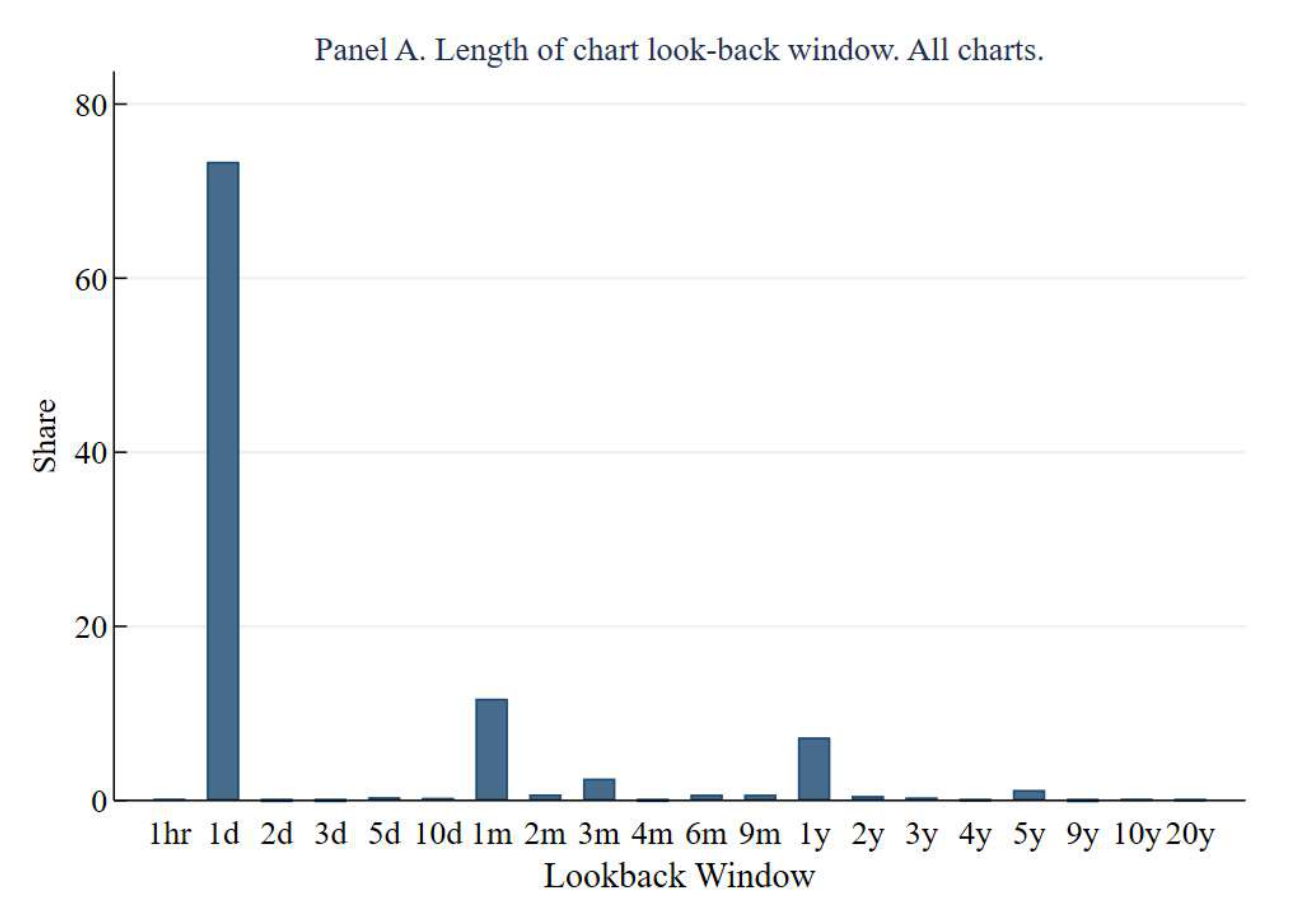
\includegraphics[width=\linewidth,height=4.72cm,keepaspectratio]{lookback-all.png}
    \column{.27\textwidth}
      \greatnum{\(>70\%\)}\par
      {\small 图表属于日内窗口}\par
      \medskip
      {\small 先定位横轴 \textbf{1d}，再读该柱在面板内的份额。}
  \end{columns}
  \refnote{Figure 1A（p.~52），p.~27。全样本，图表包含默认显示。}
\end{frame}

\begin{frame}{主动调整窗口时，常选择更长的历史}
  \strap{3.3\quad 再看主动调整者的选择}
  \begin{columns}[c,onlytextwidth]
    \column{.70\textwidth}
      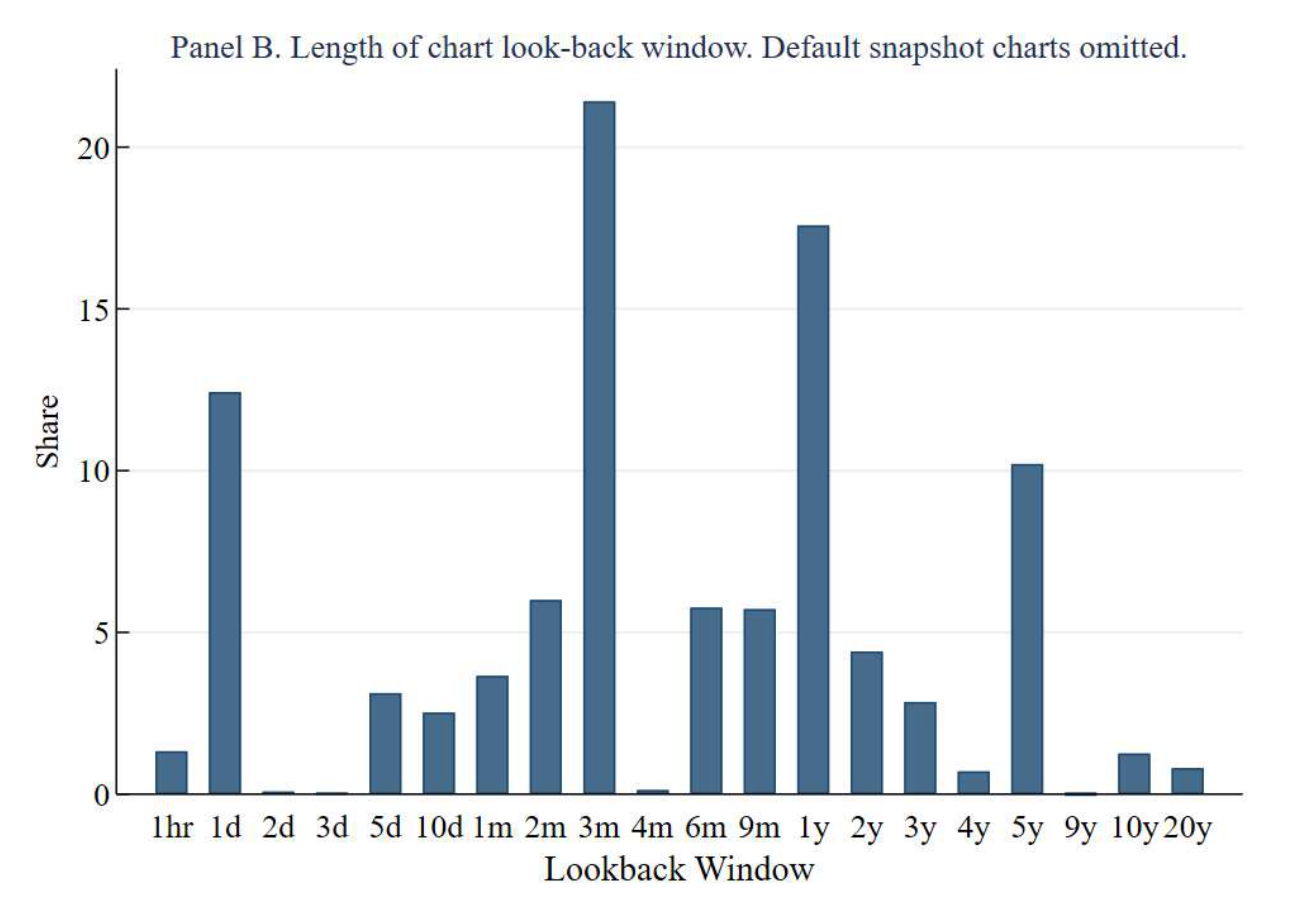
\includegraphics[width=\linewidth,height=4.72cm,keepaspectratio]{lookback-opt-in.png}
    \column{.27\textwidth}
      \textcolor{wine}{\bfseries 一个月至一年}\par
      \medskip
      {\small 先看3m和1y。两面板的分母与纵轴尺度有别。}
  \end{columns}
  \nextq{总体内容画像由哪些股票和家庭形成？}
  \refnote{Figure 1B（p.~52），p.~27。面板描述主动选择的窗口，按原图裁剪。}
\end{frame}

\section{实证比较}
\subsection{4.1 股票注意力}
\begin{frame}{“更受关注”可以指三种不同结果}
  \strap{4.1\quad 分析单位为股票×月份}
  \begin{tabularx}{\linewidth}{@{}L{.25\linewidth}Y@{}}
    \toprule
    \textbf{经济问题} & \textbf{被解释变量}\\
    \midrule
    多少人研究？ & $A$：研究该股的投资者比例。\\
    共用多少时间？ & $L=\ln(1+\text{合计分钟})$，合计分钟等于人数乘以参与者平均分钟。\\
    内容向哪侧倾斜？ & $D$：价格相关覆盖率减基本面覆盖率。同一户可进入两类。\\
    \bottomrule
  \end{tabularx}
  \smallskip
  {\small
     \textbf{价格组}\quad 价格图、技术分析\par
     \textbf{基本面组}\quad 盈利、分红、其他基本面、分析师、公司网站}
  \refnote{论文 pp.~29–32，Table 4。前1,000大CRSP股票，3,962个股票月份。}
\end{frame}

\begin{frame}{以规模为基准，再比较股票特征}
  \strap{4.1\quad 从单变量基准到扩展规格}
  \[
    Y_{jm}=\alpha+\beta\,z(\ln MC_{jm})
      +\gamma'Z_{jm}+\delta_{\mathrm{FF49}(j)}+\varepsilon_{jm}
  \]
  \begin{columns}[T,onlytextwidth]
    \column{.43\textwidth}
      \shortlabel{仅市值 · 第1列}\par
      多大程度上能用公司规模解释覆盖率？
    \column{.53\textwidth}
      \shortlabel{扩展规格 · 第3、4、6列}\par
      控制规模、股票特征和行业后，比较覆盖、时长与内容差。
  \end{columns}
  \medskip
  {\small $Y\in\{A,L,D\}$。$Z$含新闻、风险、收益及散户活动等变量。\par
  非虚拟解释变量标准化。系数对应增加一个标准差的条件关联。}
  \refnote{据 Table 4（pp.~49–50）写出扩展规格。原表采用滞后两个月的Newey–West标准误。}
\end{frame}

\begin{frame}{规模首先解释有多少人研究}
  \strap{4.1\quad 只用对数市值解释覆盖率}
  \vfill
  \begin{columns}[c,onlytextwidth]
    \column{.31\textwidth}\centering
      \greatnum{1.01\%}\par\small 原文的平均覆盖率
    \column{.36\textwidth}\centering
      {\Large\textcolor{slate}{\(\longrightarrow\)}}\par
      \small 对数市值高1个标准差
    \column{.31\textwidth}\centering
      \greatnum{2.04\%}\par\small 原文的量级示例
  \end{columns}
  \medskip
  {\small\centering \(+1.03\) 个百分点，\(t=14.42\)，\(R^2=0.315\)\par}
  \vfill
  \nextq{覆盖更广时，是否也更偏向价格信息？}
  \refnote{论文 pp.~29–31，Table 4 第1列。\(R^2\) 表示解释的样本变异比例。}
\end{frame}

\begin{frame}{覆盖、时长与内容的方向可以不同}
  \strap{4.1\quad 横读每行，比较同一特征对应的三项结果}
  {\small
  \begin{tabularx}{\linewidth}{@{}Yrrr@{}}
    \toprule
    \textbf{特征} & \textbf{$A$ 覆盖率} & \textbf{$L$ 总时长} & \textbf{$D$ 内容差}\\
     & {\scriptsize 第3列} & {\scriptsize 第4列} & {\scriptsize 第6列}\\
    \midrule
    \(\ln\)市值 & 1.13 {\scriptsize (11.35)} & 0.49 {\scriptsize (15.23)} & 0.03 {\scriptsize (0.61)}\\
    收益波动率 & 0.09 {\scriptsize (2.80)} & 0.10 {\scriptsize (5.35)} & 0.06 {\scriptsize (4.63)}\\
    \textcolor{wine}{\textbf{动量}} & \textcolor{wine}{\(-0.07\) {\scriptsize (\(-2.23\))}} &
        \textcolor{wine}{0.04 {\scriptsize (2.18)}} & \textcolor{wine}{0.05 {\scriptsize (2.33)}}\\
    分析师覆盖数 & 0.11 {\scriptsize (2.06)} & 0.04 {\scriptsize (2.07)} & \(-0.10\) {\scriptsize (\(-2.42\))}\\
    \bottomrule
  \end{tabularx}}
  \finding{动量与覆盖率负相关，与合计研究时长和相对价格覆盖正相关。}
  \refnote{Table 4（pp.~49–50）。$A,D$ 为百分点，$L$ 为对数变换。括号为原表$t$值。3,962个股票月份，包含FF49行业效应。动量窗口为$t-12$至$t-2$月。}
\end{frame}

\subsection{4.2 家庭研究风格}
\begin{frame}{哪些内容会在同一家庭一起出现？}
  \strap{4.2\quad PCA的输入与比较任务}
  \begin{tabularx}{\linewidth}{@{}L{.23\linewidth}Y@{}}
    \toprule
    \textbf{矩阵结构} & \textbf{变量}\\
    \midrule
    一行 & 一个家庭。\\
    13个主题指标 & 月均研究超过2分钟取1，否则取0。\\
    1个连续指标 & 投机标的倾向，用于观察所研究标的与主题配置怎样共同变化。\\
    \bottomrule
  \end{tabularx}
  {\small
  \textbf{主题列}\quad 综合行情、未知新闻、讨论板、盈利、分红、其他基本面、\mbox{分析师}、所有权、公司网站、价格图、技术分析、其他、无法判断。}
  \nextq{先看各类主题是否共同参与，再看内容偏好是否与标的倾向相关。}
  \refnote{论文 p.~35，Table 5（p.~51）。风险统计因参与极少而排除。横截面的完整输入矩阵未公开。}
\end{frame}

\begin{frame}{PC1主要反映跨主题的共同参与}
  \strap{4.2\quad 各主题载荷大多同向，投机标的倾向接近零}
  \centering
  \begin{tikzpicture}[x=7.45cm,y=.51cm]
    \draw[quiet!55] (0,.45)--(0,6.6);
    \foreach \y/\k/\v/\n in {6/{分析师}/.32/0.32,5/{价格图}/.31/0.31,4/{盈利}/.29/0.29,
      3/{其他基本面}/.28/0.28,2/{讨论板}/.16/0.16,1/{投机标的倾向}/.01/0.01}{
        \node[anchor=east,font=\small] at (-.016,\y) {\k};
        \fill[wine] (0,\y-.17) rectangle (\v,\y+.17);
        \node[anchor=west,font=\small,text=wine] at (\v,\y) {\n};
    }
    \node[below,font=\scriptsize] at (0,.42) {0};
    \node[anchor=west,font=\small\bfseries,text=slate] at (.52,4.9) {26.81\%};
    \node[anchor=west,font=\scriptsize,text=slate] at (.52,4.2) {解释变异份额};
  \end{tikzpicture}
  \raggedright
  \finding{高载荷落在不同主题上。PC1描述家庭是否广泛参与各类研究。}
  \refnote{据 Table 5（p.~51）选绘，保留原表符号。}
\end{frame}

\begin{frame}{PC2把内容侧重与标的倾向联系起来}
  \strap{4.2\quad 从正负两侧读这一条方向}
  \centering
  \begin{tikzpicture}[x=7.45cm,y=.45cm]
    \draw[quiet!55] (0,.35)--(0,8.45);
    \foreach \y/\k/\v/\n/\sty/\anch in {8/{讨论板}/.46/+0.46/wine/west,
      7/{投机标的倾向}/.43/+0.43/wine/west,6/{价格图}/.19/+0.19/wine/west,
      5/{分析师}/0/0.00/quiet/west,4/{技术分析}/-.11/\(-0.11\)/slate/east,
      3/{其他基本面}/-.29/\(-0.29\)/slate/east,2/{盈利}/-.34/\(-0.34\)/slate/east,
      1/{分红}/-.47/\(-0.47\)/slate/east}{
        \node[anchor=east,font=\scriptsize] at (-.63,\y) {\k};
        \fill[\sty] (0,\y-.16) rectangle (\v,\y+.16);
        \node[anchor=\anch,font=\scriptsize,text=\sty] at (\v,\y) {\n};
    }
    \node[below,font=\scriptsize] at (0,.32) {0};
  \end{tikzpicture}
  \raggedright
  \finding{PC2解释8.77\%。标的倾向参与了构造，载荷刻画联合共变。}
  \refnote{据 Table 5（p.~51）选绘。符号按原表，可整体翻转。}
\end{frame}

\subsection{4.3 交易时点}
\begin{frame}{同股研究在交易附近迅速累积}
  \begin{columns}[c,onlytextwidth]
    \column{.73\textwidth}
      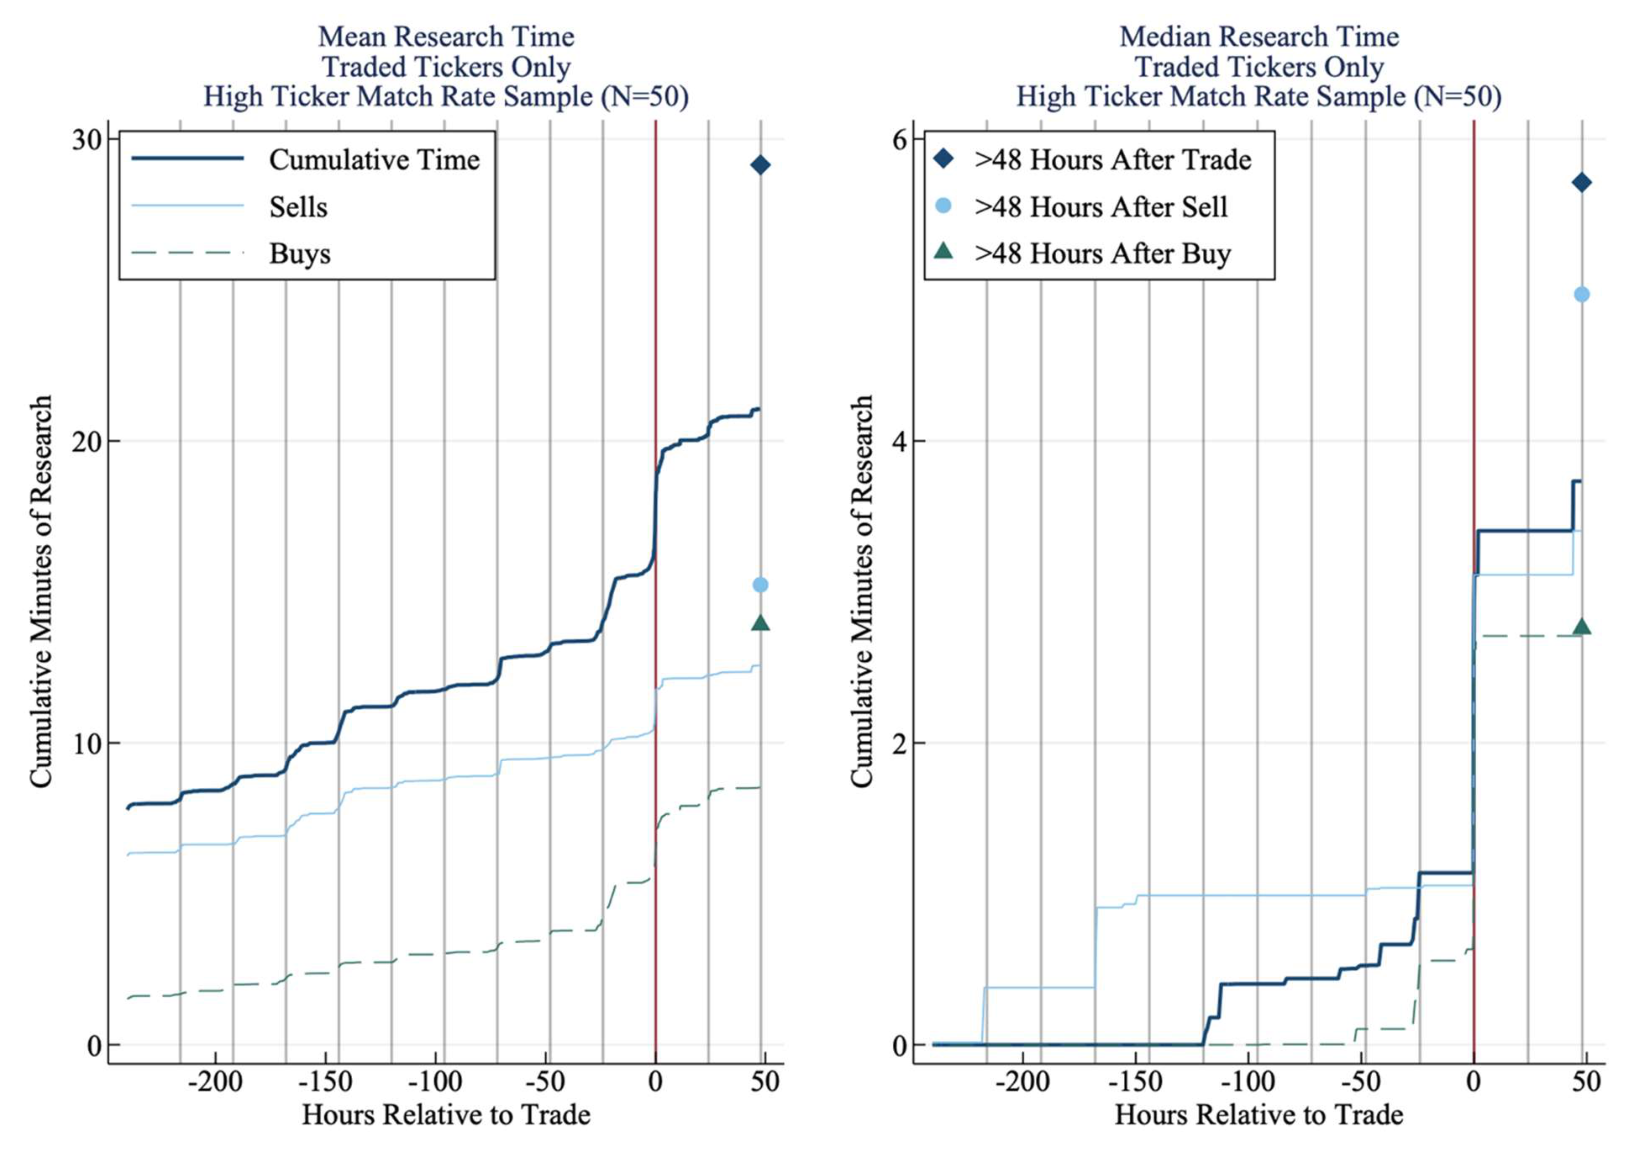
\includegraphics[width=\linewidth,height=5.15cm,keepaspectratio]{trade-timing.png}
    \column{.24\textwidth}
      \small
      \shortlabel{先看右图}\par
      中位数在交易时点附近跳升。
      \medskip\par
      \shortlabel{再看左图}\par
      均值在较早时点已有累积。
  \end{columns}
  \smallskip
  {\small 横轴为相对交易的小时，红线为0。纵轴为累计分钟，两图尺度不同。}
  \refnote{Figure 3（p.~54），50户高匹配样本。左端可含窗口前的累积，右端符号为样本期末总量。}
\end{frame}

\begin{frame}{相同的主题合计，也可以有不同的顺序}
  \strap{4.3\quad 十天内，同一主题只保留第一次出现}
  {\small
  \begin{tabular}{@{}ll@{}}
    原序列 & 价格图 → 盈利 → 分红 → 再看价格图\\
    保留后 & \textcolor{wine}{价格图 → 盈利 → 分红 → END}
  \end{tabular}\par}
  \smallskip
  \begin{columns}[c,onlytextwidth]
    \column{.72\textwidth}
      \begin{tikzpicture}
        \node[inner sep=0] (path) {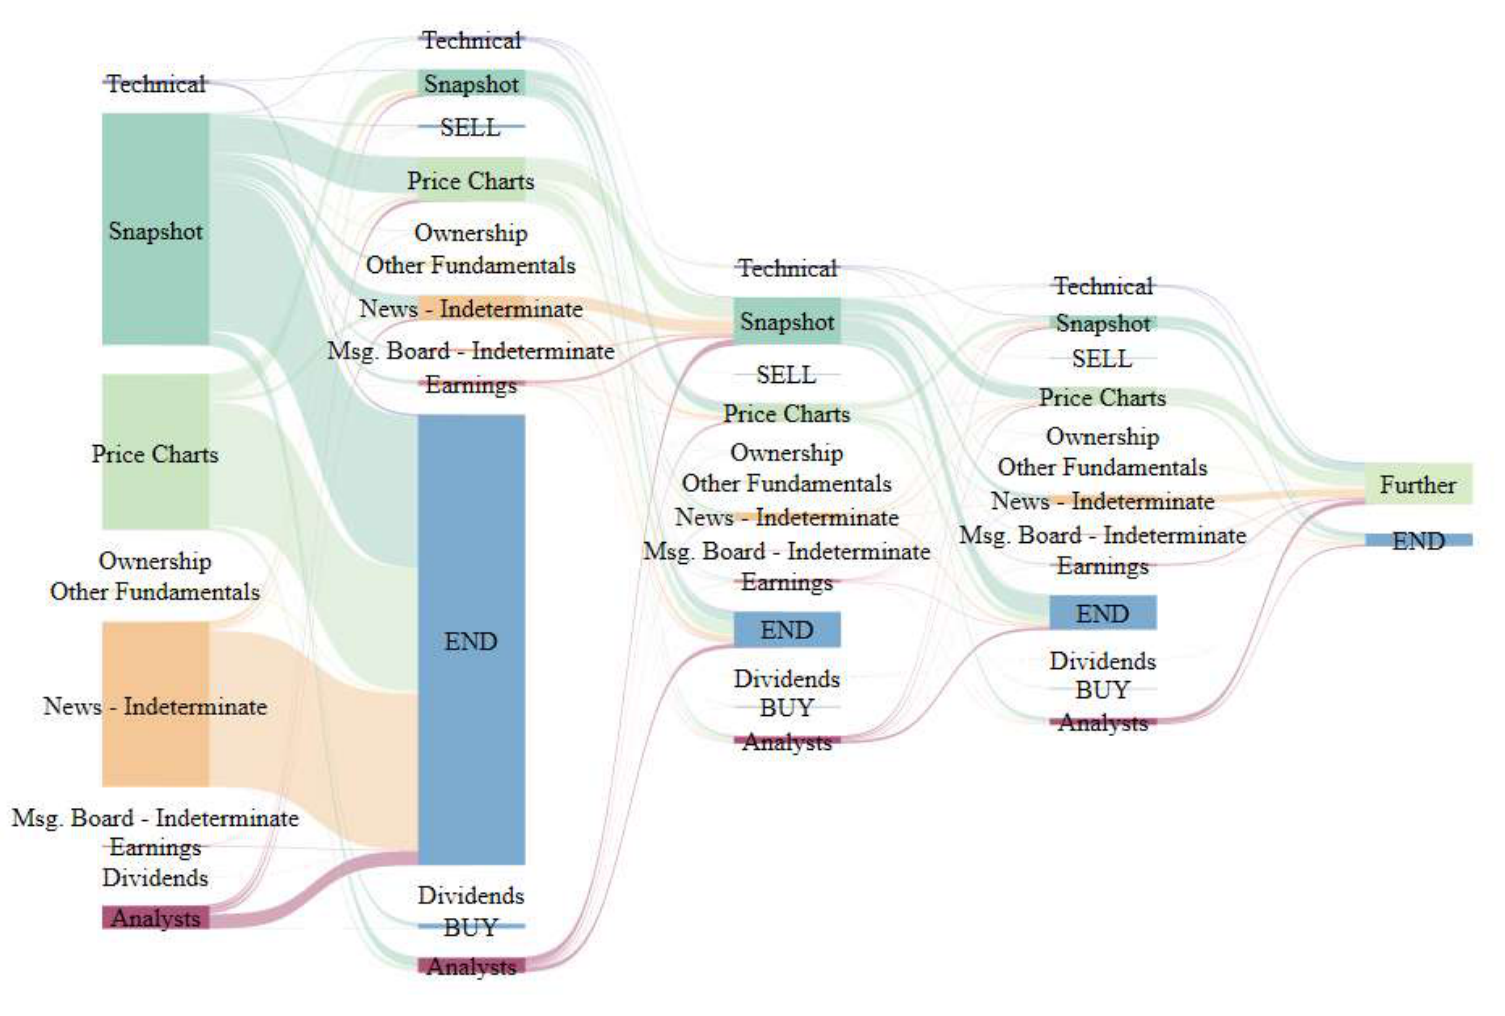
\includegraphics[width=\linewidth,height=4.26cm,keepaspectratio]{research-paths.png}};
        \draw[wine,thick,rounded corners=1pt]
           ($(path.south west)!.065!(path.south east)+(0,2.70)$) rectangle
           ($(path.south west)!.15!(path.south east)+(0,3.76)$);
        \draw[slate,thick,rounded corners=1pt]
           ($(path.south west)!.27!(path.south east)+(0,.63)$) rectangle
           ($(path.south west)!.36!(path.south east)+(0,2.56)$);
      \end{tikzpicture}
    \column{.25\textwidth}
      \small
      \shortlabel{读左边两列}\par
      酒红框：综合行情是常见入口。\par
      蓝框：第一步之后结束。
  \end{columns}
  \refnote{Figure 4（p.~55），484户、16,930个融合窗口。只留主题首次出现，线宽表示窗口数。}
\end{frame}

\begin{frame}{回看买卖之前，粗主题次序相近}
  \strap{4.3\quad 从交易端向左回看前一组主题}
  \begin{columns}[c,onlytextwidth]
    \column{.48\textwidth}\centering\shortlabel{买入前}\par
    \column{.48\textwidth}\centering\shortlabel{卖出前}\par
  \end{columns}
  \centering
  \begin{tikzpicture}
    \node[inner sep=0] (paths)
      {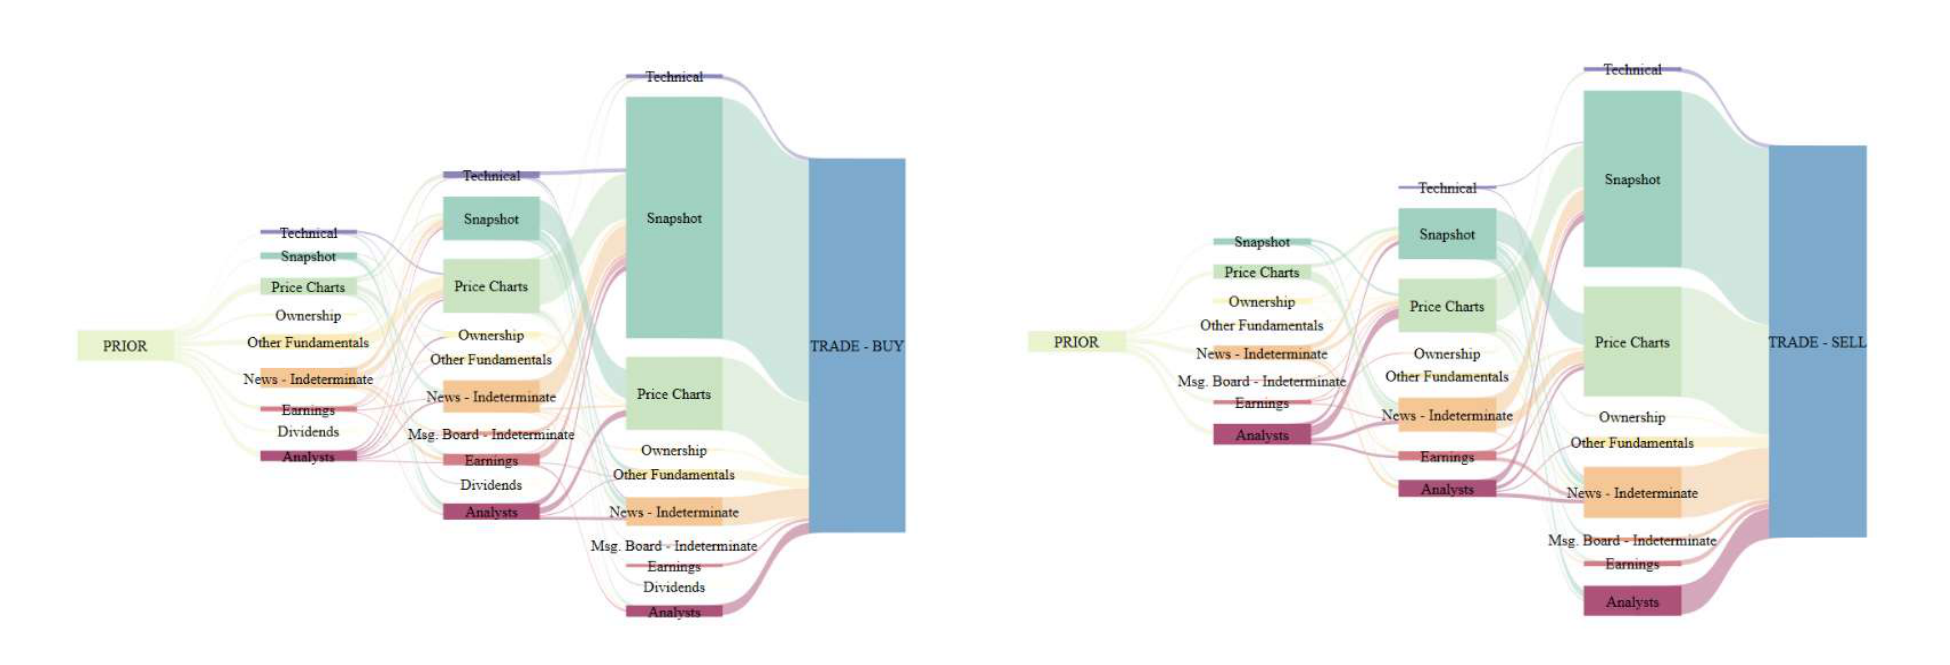
\includegraphics[width=.99\linewidth,height=4.35cm,keepaspectratio]{paths-by-direction.png}};
    \draw[wine,thick,rounded corners=1pt]
       ($(paths.south west)!.316!(paths.south east)+(0,1.39)$) rectangle
       ($(paths.south west)!.377!(paths.south east)+(0,3.37)$);
    \draw[wine,thick,rounded corners=1pt]
       ($(paths.south west)!.807!(paths.south east)+(0,1.51)$) rectangle
       ($(paths.south west)!.868!(paths.south east)+(0,3.41)$);
  \end{tikzpicture}\par
  \raggedright
  \finding{两侧临近交易处都突出综合行情和价格图。解释买卖方向还需要具体信号、先验或持仓。}
  \refnote{Figure 5 Panels A–B（p.~56）。线宽按窗口数，比较面板内的主题顺序。}
\end{frame}

\section{贡献与评价}
\subsection{5.1 主要发现}
\begin{frame}{数据为模型的信息输入提供了哪些约束？}
  \strap{5.1\quad 回到开场：投资者实际获得了什么}
  {\small\begin{tabularx}{\linewidth}{@{}L{.13\linewidth}YL{.19\linewidth}@{}}
    \toprule
    \textbf{对象} & \textbf{从数据看到的事实} & \textbf{证据}\\
    \midrule
    投入 & 典型家庭对已交易股票的可见研究有限，分布右偏。 & 表2\\
    内容 & 价格图覆盖广。默认展示和主动调整对应不同历史窗口。 & 表3、图1\\
    差异 & 股票覆盖与内容侧重有别。家庭差异体现于参与程度和主题。 & 表4–5\\
    时点 & 同股研究在交易附近集中。许多路径在一个主题后结束。 & 图3–5\\
    \bottomrule
  \end{tabularx}}
  \finding{理论可对照具体的内容、期限和获取时点，再研究它们怎样进入预期与需求。}
  \refnote{作者贡献与研究方向见论文 pp.~5–7、40–41。}
\end{frame}

\subsection{5.2 评价与后续}
\begin{frame}{页面访问可直接看见，内容占比依赖分配}
  \strap{5.2\quad 汇报人评价}
  \begin{columns}[T,onlytextwidth]
    \column{.46\textwidth}
      \shortlabel{直接分类}\par
      \greatnum{93\%}\par
      {\small 家庭访问过价格图。约1\%专门查看传统风险统计。}
    \column{.49\textwidth}
      \shortlabel{内容归因}\par
      \greatnum{\(\approx 42\%\)}\par
      {\small 均值研究分钟来自三类混合页。分配后，价格图约占44.7\%。}
  \end{columns}
  \medskip
  \finding{进一步比较不同分配权重下，主题排序是否稳定，份额变化有多大。}
  \refnote{Table 3（p.~48）、附录 pp.~66–68、Table IA2。42\%和44.7\%据表计算。}
\end{frame}

\begin{frame}{哪些实际接触的信息改变了判断？}
  \strap{5.2\quad 以默认窗口为例的后续检验}
  \begin{center}
    \begin{tikzpicture}
      \node[storyfocus,text width=2.7cm] (a) {随机改变\\默认回看窗口};
      \node[storybox,text width=2.7cm,right=6mm of a] (b) {记录实际曝光\\与主动调整};
      \node[storybox,text width=2.7cm,right=6mm of b] (c) {比较前后预期\\与后续选择};
      \draw[grapharrow] (a)--(b);
      \draw[storyarrow] (b)--(c);
    \end{tikzpicture}
  \end{center}
  \vspace{3mm}
  \finding{本文把可得资料与个体实际获取的内容区分开来。现在可以进一步检验其中哪些信号进入判断和行动。}
  \refnote{默认窗口实验为汇报人拟议设计。论文的后续问题见 p.~41。}
\end{frame}

\end{document}
